\documentclass[1p]{elsarticle_modified}
%\bibliographystyle{elsarticle-num}

%\usepackage[colorlinks]{hyperref}
%\usepackage{abbrmath_seonhwa} %\Abb, \Ascr, \Acal ,\Abf, \Afrak
\usepackage{amsfonts}
\usepackage{amssymb}
\usepackage{amsmath}
\usepackage{amsthm}
\usepackage{scalefnt}
\usepackage{amsbsy}
\usepackage{kotex}
\usepackage{caption}
\usepackage{subfig}
\usepackage{color}
\usepackage{graphicx}
\usepackage{xcolor} %% white, black, red, green, blue, cyan, magenta, yellow
\usepackage{float}
\usepackage{setspace}
\usepackage{hyperref}

\usepackage{tikz}
\usetikzlibrary{arrows}

\usepackage{multirow}
\usepackage{array} % fixed length table
\usepackage{hhline}

%%%%%%%%%%%%%%%%%%%%%
\makeatletter
\renewcommand*\env@matrix[1][\arraystretch]{%
	\edef\arraystretch{#1}%
	\hskip -\arraycolsep
	\let\@ifnextchar\new@ifnextchar
	\array{*\c@MaxMatrixCols c}}
\makeatother %https://tex.stackexchange.com/questions/14071/how-can-i-increase-the-line-spacing-in-a-matrix
%%%%%%%%%%%%%%%

\usepackage[normalem]{ulem}

\newcommand{\msout}[1]{\ifmmode\text{\sout{\ensuremath{#1}}}\else\sout{#1}\fi}
%SOURCE: \msout is \stkout macro in https://tex.stackexchange.com/questions/20609/strikeout-in-math-mode

\newcommand{\cancel}[1]{
	\ifmmode
	{\color{red}\msout{#1}}
	\else
	{\color{red}\sout{#1}}
	\fi
}

\newcommand{\add}[1]{
	{\color{blue}\uwave{#1}}
}

\newcommand{\replace}[2]{
	\ifmmode
	{\color{red}\msout{#1}}{\color{blue}\uwave{#2}}
	\else
	{\color{red}\sout{#1}}{\color{blue}\uwave{#2}}
	\fi
}

\newcommand{\Sol}{\mathcal{S}} %segment
\newcommand{\D}{D} %diagram
\newcommand{\A}{\mathcal{A}} %arc


%%%%%%%%%%%%%%%%%%%%%%%%%%%%%5 test

\def\sl{\operatorname{\textup{SL}}(2,\Cbb)}
\def\psl{\operatorname{\textup{PSL}}(2,\Cbb)}
\def\quan{\mkern 1mu \triangleright \mkern 1mu}

\theoremstyle{definition}
\newtheorem{thm}{Theorem}[section]
\newtheorem{prop}[thm]{Proposition}
\newtheorem{lem}[thm]{Lemma}
\newtheorem{ques}[thm]{Question}
\newtheorem{cor}[thm]{Corollary}
\newtheorem{defn}[thm]{Definition}
\newtheorem{exam}[thm]{Example}
\newtheorem{rmk}[thm]{Remark}
\newtheorem{alg}[thm]{Algorithm}

\newcommand{\I}{\sqrt{-1}}
\begin{document}

%\begin{frontmatter}
%
%\title{Boundary parabolic representations of knots up to 8 crossings}
%
%%% Group authors per affiliation:
%\author{Yunhi Cho} 
%\address{Department of Mathematics, University of Seoul, Seoul, Korea}
%\ead{yhcho@uos.ac.kr}
%
%
%\author{Seonhwa Kim} %\fnref{s_kim}}
%\address{Center for Geometry and Physics, Institute for Basic Science, Pohang, 37673, Korea}
%\ead{ryeona17@ibs.re.kr}
%
%\author{Hyuk Kim}
%\address{Department of Mathematical Sciences, Seoul National University, Seoul 08826, Korea}
%\ead{hyukkim@snu.ac.kr}
%
%\author{Seokbeom Yoon}
%\address{Department of Mathematical Sciences, Seoul National University, Seoul, 08826,  Korea}
%\ead{sbyoon15@snu.ac.kr}
%
%\begin{abstract}
%We find all boundary parabolic representation of knots up to 8 crossings.
%
%\end{abstract}
%\begin{keyword}
%    \MSC[2010] 57M25 
%\end{keyword}
%
%\end{frontmatter}

%\linenumbers
%\tableofcontents
%
\newcommand\colored[1]{\textcolor{white}{\rule[-0.35ex]{0.8em}{1.4ex}}\kern-0.8em\color{red} #1}%
%\newcommand\colored[1]{\textcolor{white}{ #1}\kern-2.17ex	\textcolor{white}{ #1}\kern-1.81ex	\textcolor{white}{ #1}\kern-2.15ex\color{red}#1	}

{\Large $\underline{12n_{0145}~(K12n_{0145})}$}

\setlength{\tabcolsep}{10pt}
\renewcommand{\arraystretch}{1.6}
\vspace{1cm}\begin{tabular}{m{100pt}>{\centering\arraybackslash}m{274pt}}
\multirow{5}{120pt}{
	\centering
	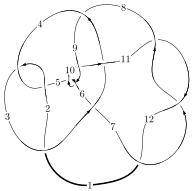
\includegraphics[width=112pt]{../../../GIT/diagram.site/Diagrams/png/2234_12n_0145.png}\\
\ \ \ A knot diagram\footnotemark}&
\allowdisplaybreaks
\textbf{Linearized knot diagam} \\
\cline{2-2}
 &
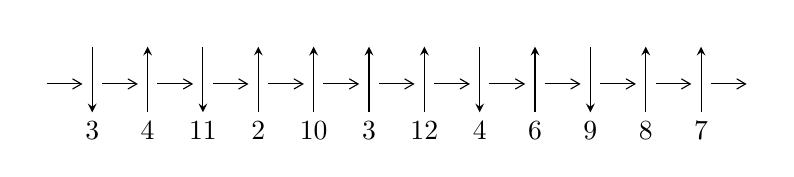
\begin{tikzpicture}[x=20pt, y=17pt]
	% nodes
	\node (C0) at (0, 0) {};
	\node (C1) at (1, 0) {};
	\node (C1U) at (1, +1) {};
	\node (C1D) at (1, -1) {3};

	\node (C2) at (2, 0) {};
	\node (C2U) at (2, +1) {};
	\node (C2D) at (2, -1) {4};

	\node (C3) at (3, 0) {};
	\node (C3U) at (3, +1) {};
	\node (C3D) at (3, -1) {11};

	\node (C4) at (4, 0) {};
	\node (C4U) at (4, +1) {};
	\node (C4D) at (4, -1) {2};

	\node (C5) at (5, 0) {};
	\node (C5U) at (5, +1) {};
	\node (C5D) at (5, -1) {10};

	\node (C6) at (6, 0) {};
	\node (C6U) at (6, +1) {};
	\node (C6D) at (6, -1) {3};

	\node (C7) at (7, 0) {};
	\node (C7U) at (7, +1) {};
	\node (C7D) at (7, -1) {12};

	\node (C8) at (8, 0) {};
	\node (C8U) at (8, +1) {};
	\node (C8D) at (8, -1) {4};

	\node (C9) at (9, 0) {};
	\node (C9U) at (9, +1) {};
	\node (C9D) at (9, -1) {6};

	\node (C10) at (10, 0) {};
	\node (C10U) at (10, +1) {};
	\node (C10D) at (10, -1) {9};

	\node (C11) at (11, 0) {};
	\node (C11U) at (11, +1) {};
	\node (C11D) at (11, -1) {8};

	\node (C12) at (12, 0) {};
	\node (C12U) at (12, +1) {};
	\node (C12D) at (12, -1) {7};
	\node (C13) at (13, 0) {};

	% arrows
	\draw[->,>={angle 60}]
	(C0) edge (C1) (C1) edge (C2) (C2) edge (C3) (C3) edge (C4) (C4) edge (C5) (C5) edge (C6) (C6) edge (C7) (C7) edge (C8) (C8) edge (C9) (C9) edge (C10) (C10) edge (C11) (C11) edge (C12) (C12) edge (C13) ;	\draw[->,>=stealth]
	(C1U) edge (C1D) (C2D) edge (C2U) (C3U) edge (C3D) (C4D) edge (C4U) (C5D) edge (C5U) (C6D) edge (C6U) (C7D) edge (C7U) (C8U) edge (C8D) (C9D) edge (C9U) (C10U) edge (C10D) (C11D) edge (C11U) (C12D) edge (C12U) ;
	\end{tikzpicture} \\
\hhline{~~} \\& 
\textbf{Solving Sequence} \\ \cline{2-2} 
 &
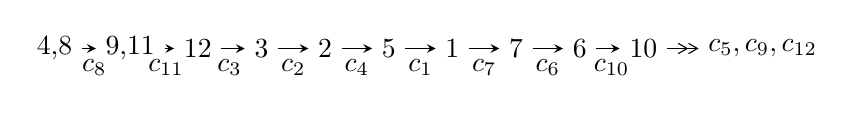
\begin{tikzpicture}[x=23pt, y=7pt]
	% node
	\node (A0) at (-1/8, 0) {4,8};
	\node (A1) at (17/16, 0) {9,11};
	\node (A2) at (17/8, 0) {12};
	\node (A3) at (25/8, 0) {3};
	\node (A4) at (33/8, 0) {2};
	\node (A5) at (41/8, 0) {5};
	\node (A6) at (49/8, 0) {1};
	\node (A7) at (57/8, 0) {7};
	\node (A8) at (65/8, 0) {6};
	\node (A9) at (73/8, 0) {10};
	\node (C1) at (1/2, -1) {$c_{8}$};
	\node (C2) at (13/8, -1) {$c_{11}$};
	\node (C3) at (21/8, -1) {$c_{3}$};
	\node (C4) at (29/8, -1) {$c_{2}$};
	\node (C5) at (37/8, -1) {$c_{4}$};
	\node (C6) at (45/8, -1) {$c_{1}$};
	\node (C7) at (53/8, -1) {$c_{7}$};
	\node (C8) at (61/8, -1) {$c_{6}$};
	\node (C9) at (69/8, -1) {$c_{10}$};
	\node (A10) at (11, 0) {$c_{5},c_{9},c_{12}$};

	% edge
	\draw[->,>=stealth]	
	(A0) edge (A1) (A1) edge (A2) (A2) edge (A3) (A3) edge (A4) (A4) edge (A5) (A5) edge (A6) (A6) edge (A7) (A7) edge (A8) (A8) edge (A9) ;
	\draw[->>,>={angle 60}]	
	(A9) edge (A10);
\end{tikzpicture} \\ 

\end{tabular} \\

\footnotetext{
The image of knot diagram is generated by the software ``\textbf{Draw programme}" developed by Andrew Bartholomew(\url{http://www.layer8.co.uk/maths/draw/index.htm\#Running-draw}), where we modified some parts for our purpose(\url{https://github.com/CATsTAILs/LinksPainter}).
}\phantom \\ \newline 
\centering \textbf{Ideals for irreducible components\footnotemark of $X_{\text{par}}$} 
 
\begin{align*}
I^u_{1}&=\langle 
-1.89198\times10^{43} u^{23}+1.93706\times10^{43} u^{22}+\cdots+7.16795\times10^{45} b+5.20518\times10^{46},\\
\phantom{I^u_{1}}&\phantom{= \langle  }-8.64361\times10^{44} u^{23}-3.86826\times10^{43} u^{22}+\cdots+2.95871\times10^{48} a+6.38636\times10^{47},\\
\phantom{I^u_{1}}&\phantom{= \langle  }u^{24}-2 u^{23}+\cdots-4461 u+2683\rangle \\
I^u_{2}&=\langle 
u^3-3 u^2+2 b+3 u-1,\;- u^3+4 u^2+6 a- u-6,\;u^4-4 u^3+4 u^2+3\rangle \\
I^u_{3}&=\langle 
b,\;a^2+a+1,\;u+1\rangle \\
I^u_{4}&=\langle 
- u^3-3 u^2+b-3 u+4,\;-3 u^3-8 u^2+3 a-8 u+12,\;u^4+2 u^3+u^2-6 u+3\rangle \\
I^u_{5}&=\langle 
b,\;a-1,\;u^2- u+1\rangle \\
\\
\end{align*}
\raggedright * 5 irreducible components of $\dim_{\mathbb{C}}=0$, with total 36 representations.\\
\footnotetext{All coefficients of polynomials are rational numbers. But the coefficients are sometimes approximated in decimal forms when there is not enough margin.}
\newpage
\renewcommand{\arraystretch}{1}
\centering \section*{I. $I^u_{1}= \langle -1.89\times10^{43} u^{23}+1.94\times10^{43} u^{22}+\cdots+7.17\times10^{45} b+5.21\times10^{46},\;-8.64\times10^{44} u^{23}-3.87\times10^{43} u^{22}+\cdots+2.96\times10^{48} a+6.39\times10^{47},\;u^{24}-2 u^{23}+\cdots-4461 u+2683 \rangle$}
\flushleft \textbf{(i) Arc colorings}\\
\begin{tabular}{m{7pt} m{180pt} m{7pt} m{180pt} }
\flushright $a_{4}=$&$\begin{pmatrix}0\\u\end{pmatrix}$ \\
\flushright $a_{8}=$&$\begin{pmatrix}1\\0\end{pmatrix}$ \\
\flushright $a_{9}=$&$\begin{pmatrix}1\\u^2\end{pmatrix}$ \\
\flushright $a_{11}=$&$\begin{pmatrix}0.000292141 u^{23}+0.0000130742 u^{22}+\cdots+0.720325 u-0.215850\\0.00263951 u^{23}-0.00270240 u^{22}+\cdots+4.46888 u-7.26175\end{pmatrix}$ \\
\flushright $a_{12}=$&$\begin{pmatrix}0.00293165 u^{23}-0.00268932 u^{22}+\cdots+5.18921 u-7.47760\\0.00263951 u^{23}-0.00270240 u^{22}+\cdots+4.46888 u-7.26175\end{pmatrix}$ \\
\flushright $a_{3}=$&$\begin{pmatrix}0.00111111 u^{23}-0.00111164 u^{22}+\cdots+2.33618 u-2.85740\\0.00144537 u^{23}-0.00161867 u^{22}+\cdots+2.86920 u-4.75166\end{pmatrix}$ \\
\flushright $a_{2}=$&$\begin{pmatrix}0.00111111 u^{23}-0.00111164 u^{22}+\cdots+2.33618 u-2.85740\\0.00274132 u^{23}-0.00268026 u^{22}+\cdots+4.84242 u-7.73137\end{pmatrix}$ \\
\flushright $a_{5}=$&$\begin{pmatrix}0.00192313 u^{23}-0.00205057 u^{22}+\cdots+3.04993 u-5.46309\\0.00295092 u^{23}-0.00292037 u^{22}+\cdots+5.36339 u-8.37266\end{pmatrix}$ \\
\flushright $a_{1}=$&$\begin{pmatrix}0.00361033 u^{23}-0.00409191 u^{22}+\cdots+6.99968 u-10.2748\\0.00380171 u^{23}-0.00433836 u^{22}+\cdots+6.92476 u-11.2245\end{pmatrix}$ \\
\flushright $a_{7}=$&$\begin{pmatrix}-0.00177479 u^{23}+0.00171084 u^{22}+\cdots-3.65352 u+4.54167\\-0.00354581 u^{23}+0.00380753 u^{22}+\cdots-6.59708 u+9.57302\end{pmatrix}$ \\
\flushright $a_{6}=$&$\begin{pmatrix}0.000894363 u^{23}-0.000991958 u^{22}+\cdots+0.953738 u-2.60877\\-0.00266810 u^{23}+0.00288557 u^{22}+\cdots-5.10145 u+7.77036\end{pmatrix}$ \\
\flushright $a_{10}=$&$\begin{pmatrix}0.00191635 u^{23}-0.00193496 u^{22}+\cdots+3.30821 u-5.87489\\0.00372145 u^{23}-0.00402551 u^{22}+\cdots+5.91212 u-10.7507\end{pmatrix}$\\&\end{tabular}
\flushleft \textbf{(ii) Obstruction class $= -1$}\\~\\
\flushleft \textbf{(iii) Cusp Shapes $= 0.00451241 u^{23}-0.00553102 u^{22}+\cdots+5.54839 u-13.6361$}\\~\\
\newpage\renewcommand{\arraystretch}{1}
\flushleft \textbf{(iv) u-Polynomials at the component}\newline \\
\begin{tabular}{m{50pt}|m{274pt}}
Crossings & \hspace{64pt}u-Polynomials at each crossing \\
\hline $$\begin{aligned}c_{1}\end{aligned}$$&$\begin{aligned}
&u^{24}+43 u^{23}+\cdots+1172 u+81
\end{aligned}$\\
\hline $$\begin{aligned}c_{2},c_{4}\end{aligned}$$&$\begin{aligned}
&u^{24}-3 u^{23}+\cdots-68 u+9
\end{aligned}$\\
\hline $$\begin{aligned}c_{3}\end{aligned}$$&$\begin{aligned}
&u^{24}+3 u^{23}+\cdots-4 u+3
\end{aligned}$\\
\hline $$\begin{aligned}c_{5},c_{9}\end{aligned}$$&$\begin{aligned}
&u^{24}-3 u^{23}+\cdots+10 u+3
\end{aligned}$\\
\hline $$\begin{aligned}c_{6}\end{aligned}$$&$\begin{aligned}
&u^{24}+2 u^{23}+\cdots+20857 u+9299
\end{aligned}$\\
\hline $$\begin{aligned}c_{7},c_{11},c_{12}\end{aligned}$$&$\begin{aligned}
&u^{24}+u^{23}+\cdots-32 u+16
\end{aligned}$\\
\hline $$\begin{aligned}c_{8}\end{aligned}$$&$\begin{aligned}
&u^{24}-2 u^{23}+\cdots-4461 u+2683
\end{aligned}$\\
\hline $$\begin{aligned}c_{10}\end{aligned}$$&$\begin{aligned}
&u^{24}+19 u^{23}+\cdots+68 u+9
\end{aligned}$\\
\hline
\end{tabular}\\~\\
\newpage\renewcommand{\arraystretch}{1}
\flushleft \textbf{(v) Riley Polynomials at the component}\newline \\
\begin{tabular}{m{50pt}|m{274pt}}
Crossings & \hspace{64pt}Riley Polynomials at each crossing \\
\hline $$\begin{aligned}c_{1}\end{aligned}$$&$\begin{aligned}
&y^{24}-117 y^{23}+\cdots-1128316 y+6561
\end{aligned}$\\
\hline $$\begin{aligned}c_{2},c_{4}\end{aligned}$$&$\begin{aligned}
&y^{24}+43 y^{23}+\cdots+1172 y+81
\end{aligned}$\\
\hline $$\begin{aligned}c_{3}\end{aligned}$$&$\begin{aligned}
&y^{24}+3 y^{23}+\cdots+68 y+9
\end{aligned}$\\
\hline $$\begin{aligned}c_{5},c_{9}\end{aligned}$$&$\begin{aligned}
&y^{24}+19 y^{23}+\cdots+68 y+9
\end{aligned}$\\
\hline $$\begin{aligned}c_{6}\end{aligned}$$&$\begin{aligned}
&y^{24}+82 y^{23}+\cdots+1135326279 y+86471401
\end{aligned}$\\
\hline $$\begin{aligned}c_{7},c_{11},c_{12}\end{aligned}$$&$\begin{aligned}
&y^{24}+41 y^{23}+\cdots+2048 y+256
\end{aligned}$\\
\hline $$\begin{aligned}c_{8}\end{aligned}$$&$\begin{aligned}
&y^{24}-34 y^{23}+\cdots-21038113 y+7198489
\end{aligned}$\\
\hline $$\begin{aligned}c_{10}\end{aligned}$$&$\begin{aligned}
&y^{24}-21 y^{23}+\cdots+5492 y+81
\end{aligned}$\\
\hline
\end{tabular}\\~\\
\newpage\flushleft \textbf{(vi) Complex Volumes and Cusp Shapes}
$$\begin{array}{c|c|c}  
\text{Solutions to }I^u_{1}& \I (\text{vol} + \sqrt{-1}CS) & \text{Cusp shape}\\
 \hline 
\begin{aligned}
u &= \phantom{-}0.232862 + 0.947035 I \\
a &= -0.649985 - 0.077686 I \\
b &= \phantom{-}0.374440 + 0.304409 I\end{aligned}
 & \phantom{-}0.779807 + 1.048970 I & \phantom{-}7.25519 - 5.58365 I \\ \hline\begin{aligned}
u &= \phantom{-}0.232862 - 0.947035 I \\
a &= -0.649985 + 0.077686 I \\
b &= \phantom{-}0.374440 - 0.304409 I\end{aligned}
 & \phantom{-}0.779807 - 1.048970 I & \phantom{-}7.25519 + 5.58365 I \\ \hline\begin{aligned}
u &= \phantom{-}0.943560 + 0.064690 I \\
a &= \phantom{-}0.988902 + 0.233923 I \\
b &= -0.682289 + 0.802318 I\end{aligned}
 & -3.89306 - 0.24557 I & -2.31984 + 1.35715 I \\ \hline\begin{aligned}
u &= \phantom{-}0.943560 - 0.064690 I \\
a &= \phantom{-}0.988902 - 0.233923 I \\
b &= -0.682289 - 0.802318 I\end{aligned}
 & -3.89306 + 0.24557 I & -2.31984 - 1.35715 I \\ \hline\begin{aligned}
u &= -0.959379 + 0.455770 I \\
a &= \phantom{-}0.646370 - 0.274793 I \\
b &= -0.415041 + 0.335328 I\end{aligned}
 & -0.27313 + 3.15044 I & \phantom{-}2.29434 - 0.19419 I \\ \hline\begin{aligned}
u &= -0.959379 - 0.455770 I \\
a &= \phantom{-}0.646370 + 0.274793 I \\
b &= -0.415041 - 0.335328 I\end{aligned}
 & -0.27313 - 3.15044 I & \phantom{-}2.29434 + 0.19419 I \\ \hline\begin{aligned}
u &= -0.502276 + 0.647230 I \\
a &= -0.990775 + 0.287392 I \\
b &= \phantom{-}0.278387 + 0.380293 I\end{aligned}
 & \phantom{-}0.422299 + 1.283840 I & \phantom{-}4.39270 - 6.02370 I \\ \hline\begin{aligned}
u &= -0.502276 - 0.647230 I \\
a &= -0.990775 - 0.287392 I \\
b &= \phantom{-}0.278387 - 0.380293 I\end{aligned}
 & \phantom{-}0.422299 - 1.283840 I & \phantom{-}4.39270 + 6.02370 I \\ \hline\begin{aligned}
u &= \phantom{-}0.933542 + 0.786148 I \\
a &= -0.749432 - 0.148046 I \\
b &= \phantom{-}0.084838 - 1.367360 I\end{aligned}
 & -4.97420 - 2.33173 I & -0.59644 + 2.89442 I \\ \hline\begin{aligned}
u &= \phantom{-}0.933542 - 0.786148 I \\
a &= -0.749432 + 0.148046 I \\
b &= \phantom{-}0.084838 + 1.367360 I\end{aligned}
 & -4.97420 + 2.33173 I & -0.59644 - 2.89442 I\\
 \hline 
 \end{array}$$\newpage$$\begin{array}{c|c|c}  
\text{Solutions to }I^u_{1}& \I (\text{vol} + \sqrt{-1}CS) & \text{Cusp shape}\\
 \hline 
\begin{aligned}
u &= \phantom{-}0.607235 + 1.070690 I \\
a &= -0.470711 + 0.110611 I \\
b &= \phantom{-}0.07764 - 1.45718 I\end{aligned}
 & -4.85669 - 2.39093 I & \phantom{-}0.84102 + 2.37108 I \\ \hline\begin{aligned}
u &= \phantom{-}0.607235 - 1.070690 I \\
a &= -0.470711 - 0.110611 I \\
b &= \phantom{-}0.07764 + 1.45718 I\end{aligned}
 & -4.85669 + 2.39093 I & \phantom{-}0.84102 - 2.37108 I \\ \hline\begin{aligned}
u &= \phantom{-}1.21724 + 0.74996 I \\
a &= \phantom{-}0.400953 - 1.002140 I \\
b &= \phantom{-}0.15154 - 2.05062 I\end{aligned}
 & \phantom{-}15.8709 - 2.8783 I & -1.59016 + 0.69856 I \\ \hline\begin{aligned}
u &= \phantom{-}1.21724 - 0.74996 I \\
a &= \phantom{-}0.400953 + 1.002140 I \\
b &= \phantom{-}0.15154 + 2.05062 I\end{aligned}
 & \phantom{-}15.8709 + 2.8783 I & -1.59016 - 0.69856 I \\ \hline\begin{aligned}
u &= \phantom{-}1.52531 + 0.37916 I \\
a &= \phantom{-}0.108996 - 0.705821 I \\
b &= \phantom{-}0.138338 - 0.696834 I\end{aligned}
 & -1.17892 + 4.17832 I & -0.72824 - 4.64199 I \\ \hline\begin{aligned}
u &= \phantom{-}1.52531 - 0.37916 I \\
a &= \phantom{-}0.108996 + 0.705821 I \\
b &= \phantom{-}0.138338 + 0.696834 I\end{aligned}
 & -1.17892 - 4.17832 I & -0.72824 + 4.64199 I \\ \hline\begin{aligned}
u &= -1.78012 + 0.29967 I \\
a &= -0.680725 + 0.483351 I \\
b &= \phantom{-}0.08900 + 1.95850 I\end{aligned}
 & -18.4389 + 3.9255 I & \phantom{-}0.72969 - 1.86370 I \\ \hline\begin{aligned}
u &= -1.78012 - 0.29967 I \\
a &= -0.680725 - 0.483351 I \\
b &= \phantom{-}0.08900 - 1.95850 I\end{aligned}
 & -18.4389 - 3.9255 I & \phantom{-}0.72969 + 1.86370 I \\ \hline\begin{aligned}
u &= -1.82828 + 0.75998 I \\
a &= \phantom{-}0.679108 - 0.172953 I \\
b &= -0.71021 - 1.48438 I\end{aligned}
 & -10.81740 + 5.66544 I & -1.94284 - 3.68332 I \\ \hline\begin{aligned}
u &= -1.82828 - 0.75998 I \\
a &= \phantom{-}0.679108 + 0.172953 I \\
b &= -0.71021 + 1.48438 I\end{aligned}
 & -10.81740 - 5.66544 I & -1.94284 + 3.68332 I\\
 \hline 
 \end{array}$$\newpage$$\begin{array}{c|c|c}  
\text{Solutions to }I^u_{1}& \I (\text{vol} + \sqrt{-1}CS) & \text{Cusp shape}\\
 \hline 
\begin{aligned}
u &= -1.85631 + 0.81470 I \\
a &= \phantom{-}0.104205 + 0.704147 I \\
b &= \phantom{-}0.40009 + 1.66939 I\end{aligned}
 & -9.33657 - 1.50490 I & -1.60303 + 1.18708 I \\ \hline\begin{aligned}
u &= -1.85631 - 0.81470 I \\
a &= \phantom{-}0.104205 - 0.704147 I \\
b &= \phantom{-}0.40009 - 1.66939 I\end{aligned}
 & -9.33657 + 1.50490 I & -1.60303 - 1.18708 I \\ \hline\begin{aligned}
u &= \phantom{-}2.46660 + 0.93685 I \\
a &= \phantom{-}0.504632 + 0.296006 I \\
b &= -0.28674 + 1.91373 I\end{aligned}
 & \phantom{-}16.9567 - 10.8896 I & \phantom{-0.000000 -}0. + 4.72097 I \\ \hline\begin{aligned}
u &= \phantom{-}2.46660 - 0.93685 I \\
a &= \phantom{-}0.504632 - 0.296006 I \\
b &= -0.28674 - 1.91373 I\end{aligned}
 & \phantom{-}16.9567 + 10.8896 I & \phantom{-0.000000 } 0. - 4.72097 I\\
 \hline 
 \end{array}$$\newpage\newpage\renewcommand{\arraystretch}{1}
\centering \section*{II. $I^u_{2}= \langle u^3-3 u^2+2 b+3 u-1,\;- u^3+4 u^2+6 a- u-6,\;u^4-4 u^3+4 u^2+3 \rangle$}
\flushleft \textbf{(i) Arc colorings}\\
\begin{tabular}{m{7pt} m{180pt} m{7pt} m{180pt} }
\flushright $a_{4}=$&$\begin{pmatrix}0\\u\end{pmatrix}$ \\
\flushright $a_{8}=$&$\begin{pmatrix}1\\0\end{pmatrix}$ \\
\flushright $a_{9}=$&$\begin{pmatrix}1\\u^2\end{pmatrix}$ \\
\flushright $a_{11}=$&$\begin{pmatrix}\frac{1}{6} u^3-\frac{2}{3} u^2+\frac{1}{6} u+1\\-\frac{1}{2} u^3+\frac{3}{2} u^2-\frac{3}{2} u+\frac{1}{2}\end{pmatrix}$ \\
\flushright $a_{12}=$&$\begin{pmatrix}-\frac{1}{3} u^3+\frac{5}{6} u^2-\frac{4}{3} u+\frac{3}{2}\\-\frac{1}{2} u^3+\frac{3}{2} u^2-\frac{3}{2} u+\frac{1}{2}\end{pmatrix}$ \\
\flushright $a_{3}=$&$\begin{pmatrix}\frac{1}{6} u^3-\frac{2}{3} u^2+\frac{7}{6} u-1\\\frac{1}{2} u^3-\frac{3}{2} u^2+\frac{3}{2} u+\frac{1}{2}\end{pmatrix}$ \\
\flushright $a_{2}=$&$\begin{pmatrix}\frac{1}{6} u^3-\frac{2}{3} u^2+\frac{7}{6} u-1\\u^3-\frac{5}{2} u^2+u+\frac{1}{2}\end{pmatrix}$ \\
\flushright $a_{5}=$&$\begin{pmatrix}\frac{1}{6} u^3-\frac{2}{3} u^2+\frac{1}{6} u+1\\-\frac{1}{2} u^3+\frac{3}{2} u^2-\frac{3}{2} u+\frac{1}{2}\end{pmatrix}$ \\
\flushright $a_{1}=$&$\begin{pmatrix}-\frac{1}{6} u^3+\frac{2}{3} u^2-\frac{1}{6} u-1\\\frac{1}{2} u^3-\frac{3}{2} u^2+\frac{3}{2} u-\frac{1}{2}\end{pmatrix}$ \\
\flushright $a_{7}=$&$\begin{pmatrix}-\frac{1}{6} u^3+\frac{7}{6} u^2-\frac{13}{6} u-\frac{1}{2}\\-2\end{pmatrix}$ \\
\flushright $a_{6}=$&$\begin{pmatrix}-\frac{1}{6} u^3+\frac{2}{3} u^2-\frac{7}{6} u\\-\frac{1}{2} u^3+\frac{1}{2} u^2-\frac{1}{2} u-\frac{1}{2}\end{pmatrix}$ \\
\flushright $a_{10}=$&$\begin{pmatrix}\frac{1}{6} u^3-\frac{1}{6} u^2-\frac{5}{6} u+\frac{3}{2}\\\frac{1}{2} u^3-\frac{3}{2} u-1\end{pmatrix}$\\&\end{tabular}
\flushleft \textbf{(ii) Obstruction class $= 1$}\\~\\
\flushleft \textbf{(iii) Cusp Shapes $= 4 u^2-8 u$}\\~\\
\newpage\renewcommand{\arraystretch}{1}
\flushleft \textbf{(iv) u-Polynomials at the component}\newline \\
\begin{tabular}{m{50pt}|m{274pt}}
Crossings & \hspace{64pt}u-Polynomials at each crossing \\
\hline $$\begin{aligned}c_{1},c_{3},c_{4}\\c_{5}\end{aligned}$$&$\begin{aligned}
&(u^2- u+1)^2
\end{aligned}$\\
\hline $$\begin{aligned}c_{2},c_{9},c_{10}\end{aligned}$$&$\begin{aligned}
&(u^2+u+1)^2
\end{aligned}$\\
\hline $$\begin{aligned}c_{6}\end{aligned}$$&$\begin{aligned}
&u^4+4 u^3+4 u^2+3
\end{aligned}$\\
\hline $$\begin{aligned}c_{7},c_{11},c_{12}\end{aligned}$$&$\begin{aligned}
&(u^2+2)^2
\end{aligned}$\\
\hline $$\begin{aligned}c_{8}\end{aligned}$$&$\begin{aligned}
&u^4-4 u^3+4 u^2+3
\end{aligned}$\\
\hline
\end{tabular}\\~\\
\newpage\renewcommand{\arraystretch}{1}
\flushleft \textbf{(v) Riley Polynomials at the component}\newline \\
\begin{tabular}{m{50pt}|m{274pt}}
Crossings & \hspace{64pt}Riley Polynomials at each crossing \\
\hline $$\begin{aligned}c_{1},c_{2},c_{3}\\c_{4},c_{5},c_{9}\\c_{10}\end{aligned}$$&$\begin{aligned}
&(y^2+y+1)^2
\end{aligned}$\\
\hline $$\begin{aligned}c_{6},c_{8}\end{aligned}$$&$\begin{aligned}
&y^4-8 y^3+22 y^2+24 y+9
\end{aligned}$\\
\hline $$\begin{aligned}c_{7},c_{11},c_{12}\end{aligned}$$&$\begin{aligned}
&(y+2)^4
\end{aligned}$\\
\hline
\end{tabular}\\~\\
\newpage\flushleft \textbf{(vi) Complex Volumes and Cusp Shapes}
$$\begin{array}{c|c|c}  
\text{Solutions to }I^u_{2}& \I (\text{vol} + \sqrt{-1}CS) & \text{Cusp shape}\\
 \hline 
\begin{aligned}
u &= -0.224745 + 0.707107 I \\
a &= \phantom{-}1.316500 + 0.288675 I \\
b &= \phantom{-0.000000 } -1.414210 I\end{aligned}
 & -4.93480 + 4.05977 I & \phantom{-0.000000 } 0. - 6.92820 I \\ \hline\begin{aligned}
u &= -0.224745 - 0.707107 I \\
a &= \phantom{-}1.316500 - 0.288675 I \\
b &= \phantom{-0.000000 -}1.414210 I\end{aligned}
 & -4.93480 - 4.05977 I & \phantom{-0.000000 -}0. + 6.92820 I \\ \hline\begin{aligned}
u &= \phantom{-}2.22474 + 0.70711 I \\
a &= -0.316497 - 0.288675 I \\
b &= \phantom{-0.000000 } -1.414210 I\end{aligned}
 & -4.93480 - 4.05977 I & \phantom{-0.000000 -}0. + 6.92820 I \\ \hline\begin{aligned}
u &= \phantom{-}2.22474 - 0.70711 I \\
a &= -0.316497 + 0.288675 I \\
b &= \phantom{-0.000000 -}1.414210 I\end{aligned}
 & -4.93480 + 4.05977 I & \phantom{-0.000000 } 0. - 6.92820 I\\
 \hline 
 \end{array}$$\newpage\newpage\renewcommand{\arraystretch}{1}
\centering \section*{III. $I^u_{3}= \langle b,\;a^2+a+1,\;u+1 \rangle$}
\flushleft \textbf{(i) Arc colorings}\\
\begin{tabular}{m{7pt} m{180pt} m{7pt} m{180pt} }
\flushright $a_{4}=$&$\begin{pmatrix}0\\-1\end{pmatrix}$ \\
\flushright $a_{8}=$&$\begin{pmatrix}1\\0\end{pmatrix}$ \\
\flushright $a_{9}=$&$\begin{pmatrix}1\\1\end{pmatrix}$ \\
\flushright $a_{11}=$&$\begin{pmatrix}a\\0\end{pmatrix}$ \\
\flushright $a_{12}=$&$\begin{pmatrix}a\\0\end{pmatrix}$ \\
\flushright $a_{3}=$&$\begin{pmatrix}a+1\\-1\end{pmatrix}$ \\
\flushright $a_{2}=$&$\begin{pmatrix}a+1\\a\end{pmatrix}$ \\
\flushright $a_{5}=$&$\begin{pmatrix}- a\\0\end{pmatrix}$ \\
\flushright $a_{1}=$&$\begin{pmatrix}a\\0\end{pmatrix}$ \\
\flushright $a_{7}=$&$\begin{pmatrix}1\\0\end{pmatrix}$ \\
\flushright $a_{6}=$&$\begin{pmatrix}- a\\1\end{pmatrix}$ \\
\flushright $a_{10}=$&$\begin{pmatrix}0\\- a\end{pmatrix}$\\&\end{tabular}
\flushleft \textbf{(ii) Obstruction class $= 1$}\\~\\
\flushleft \textbf{(iii) Cusp Shapes $= -8 a+2$}\\~\\
\newpage\renewcommand{\arraystretch}{1}
\flushleft \textbf{(iv) u-Polynomials at the component}\newline \\
\begin{tabular}{m{50pt}|m{274pt}}
Crossings & \hspace{64pt}u-Polynomials at each crossing \\
\hline $$\begin{aligned}c_{1},c_{4},c_{9}\end{aligned}$$&$\begin{aligned}
&u^2- u+1
\end{aligned}$\\
\hline $$\begin{aligned}c_{2},c_{3},c_{5}\\c_{10}\end{aligned}$$&$\begin{aligned}
&u^2+u+1
\end{aligned}$\\
\hline $$\begin{aligned}c_{6},c_{8}\end{aligned}$$&$\begin{aligned}
&(u+1)^2
\end{aligned}$\\
\hline $$\begin{aligned}c_{7},c_{11},c_{12}\end{aligned}$$&$\begin{aligned}
&u^2
\end{aligned}$\\
\hline
\end{tabular}\\~\\
\newpage\renewcommand{\arraystretch}{1}
\flushleft \textbf{(v) Riley Polynomials at the component}\newline \\
\begin{tabular}{m{50pt}|m{274pt}}
Crossings & \hspace{64pt}Riley Polynomials at each crossing \\
\hline $$\begin{aligned}c_{1},c_{2},c_{3}\\c_{4},c_{5},c_{9}\\c_{10}\end{aligned}$$&$\begin{aligned}
&y^2+y+1
\end{aligned}$\\
\hline $$\begin{aligned}c_{6},c_{8}\end{aligned}$$&$\begin{aligned}
&(y-1)^2
\end{aligned}$\\
\hline $$\begin{aligned}c_{7},c_{11},c_{12}\end{aligned}$$&$\begin{aligned}
&y^2
\end{aligned}$\\
\hline
\end{tabular}\\~\\
\newpage\flushleft \textbf{(vi) Complex Volumes and Cusp Shapes}
$$\begin{array}{c|c|c}  
\text{Solutions to }I^u_{3}& \I (\text{vol} + \sqrt{-1}CS) & \text{Cusp shape}\\
 \hline 
\begin{aligned}
u &= -1.00000\phantom{ +0.000000I} \\
a &= -0.500000 + 0.866025 I \\
b &= \phantom{-0.000000 } 0\end{aligned}
 & \phantom{-0.000000 -}4.05977 I & \phantom{-}6.00000 - 6.92820 I \\ \hline\begin{aligned}
u &= -1.00000\phantom{ +0.000000I} \\
a &= -0.500000 - 0.866025 I \\
b &= \phantom{-0.000000 } 0\end{aligned}
 & \phantom{-0.000000 } -4.05977 I & \phantom{-}6.00000 + 6.92820 I\\
 \hline 
 \end{array}$$\newpage\newpage\renewcommand{\arraystretch}{1}
\centering \section*{IV. $I^u_{4}= \langle - u^3-3 u^2+b-3 u+4,\;-3 u^3-8 u^2+3 a-8 u+12,\;u^4+2 u^3+u^2-6 u+3 \rangle$}
\flushleft \textbf{(i) Arc colorings}\\
\begin{tabular}{m{7pt} m{180pt} m{7pt} m{180pt} }
\flushright $a_{4}=$&$\begin{pmatrix}0\\u\end{pmatrix}$ \\
\flushright $a_{8}=$&$\begin{pmatrix}1\\0\end{pmatrix}$ \\
\flushright $a_{9}=$&$\begin{pmatrix}1\\u^2\end{pmatrix}$ \\
\flushright $a_{11}=$&$\begin{pmatrix}u^3+\frac{8}{3} u^2+\frac{8}{3} u-4\\u^3+3 u^2+3 u-4\end{pmatrix}$ \\
\flushright $a_{12}=$&$\begin{pmatrix}2 u^3+\frac{17}{3} u^2+\frac{17}{3} u-8\\u^3+3 u^2+3 u-4\end{pmatrix}$ \\
\flushright $a_{3}=$&$\begin{pmatrix}-\frac{2}{3} u^3-2 u^2-\frac{7}{3} u+2\\-\frac{1}{3} u^3-\frac{4}{3} u^2- u+1\end{pmatrix}$ \\
\flushright $a_{2}=$&$\begin{pmatrix}-\frac{2}{3} u^3-2 u^2-\frac{7}{3} u+2\\-\frac{2}{3} u^3-\frac{8}{3} u^2-3 u+3\end{pmatrix}$ \\
\flushright $a_{5}=$&$\begin{pmatrix}u^3+\frac{8}{3} u^2+\frac{8}{3} u-4\\u^3+3 u^2+3 u-4\end{pmatrix}$ \\
\flushright $a_{1}=$&$\begin{pmatrix}- u^3-\frac{8}{3} u^2-\frac{8}{3} u+4\\- u^3-3 u^2-3 u+4\end{pmatrix}$ \\
\flushright $a_{7}=$&$\begin{pmatrix}-\frac{1}{3} u^3- u^2-\frac{5}{3} u-1\\-2\end{pmatrix}$ \\
\flushright $a_{6}=$&$\begin{pmatrix}\frac{1}{3} u^3+\frac{2}{3} u^2+\frac{1}{3} u-3\\\frac{2}{3} u^3+\frac{2}{3} u^2+u-3\end{pmatrix}$ \\
\flushright $a_{10}=$&$\begin{pmatrix}\frac{5}{3} u^3+\frac{13}{3} u^2+\frac{14}{3} u-6\\\frac{5}{3} u^3+\frac{14}{3} u^2+3 u-5\end{pmatrix}$\\&\end{tabular}
\flushleft \textbf{(ii) Obstruction class $= 1$}\\~\\
\flushleft \textbf{(iii) Cusp Shapes $= 0$}\\~\\
\newpage\renewcommand{\arraystretch}{1}
\flushleft \textbf{(iv) u-Polynomials at the component}\newline \\
\begin{tabular}{m{50pt}|m{274pt}}
Crossings & \hspace{64pt}u-Polynomials at each crossing \\
\hline $$\begin{aligned}c_{1},c_{3},c_{4}\\c_{5}\end{aligned}$$&$\begin{aligned}
&(u^2- u+1)^2
\end{aligned}$\\
\hline $$\begin{aligned}c_{2},c_{9},c_{10}\end{aligned}$$&$\begin{aligned}
&(u^2+u+1)^2
\end{aligned}$\\
\hline $$\begin{aligned}c_{6}\end{aligned}$$&$\begin{aligned}
&u^4-2 u^3+u^2+6 u+3
\end{aligned}$\\
\hline $$\begin{aligned}c_{7},c_{11},c_{12}\end{aligned}$$&$\begin{aligned}
&(u^2+2)^2
\end{aligned}$\\
\hline $$\begin{aligned}c_{8}\end{aligned}$$&$\begin{aligned}
&u^4+2 u^3+u^2-6 u+3
\end{aligned}$\\
\hline
\end{tabular}\\~\\
\newpage\renewcommand{\arraystretch}{1}
\flushleft \textbf{(v) Riley Polynomials at the component}\newline \\
\begin{tabular}{m{50pt}|m{274pt}}
Crossings & \hspace{64pt}Riley Polynomials at each crossing \\
\hline $$\begin{aligned}c_{1},c_{2},c_{3}\\c_{4},c_{5},c_{9}\\c_{10}\end{aligned}$$&$\begin{aligned}
&(y^2+y+1)^2
\end{aligned}$\\
\hline $$\begin{aligned}c_{6},c_{8}\end{aligned}$$&$\begin{aligned}
&y^4-2 y^3+31 y^2-30 y+9
\end{aligned}$\\
\hline $$\begin{aligned}c_{7},c_{11},c_{12}\end{aligned}$$&$\begin{aligned}
&(y+2)^4
\end{aligned}$\\
\hline
\end{tabular}\\~\\
\newpage\flushleft \textbf{(vi) Complex Volumes and Cusp Shapes}
$$\begin{array}{c|c|c}  
\text{Solutions to }I^u_{4}& \I (\text{vol} + \sqrt{-1}CS) & \text{Cusp shape}\\
 \hline 
\begin{aligned}
u &= \phantom{-}0.724745 + 0.158919 I \\
a &= -0.408248 + 1.284460 I \\
b &= \phantom{-0.000000 -}1.414210 I\end{aligned}
 & -4.93480\phantom{ +0.000000I} & \phantom{-0.000000 } 0 \\ \hline\begin{aligned}
u &= \phantom{-}0.724745 - 0.158919 I \\
a &= -0.408248 - 1.284460 I \\
b &= \phantom{-0.000000 } -1.414210 I\end{aligned}
 & -4.93480\phantom{ +0.000000I} & \phantom{-0.000000 } 0 \\ \hline\begin{aligned}
u &= -1.72474 + 1.57313 I \\
a &= \phantom{-}0.408248 - 0.129757 I \\
b &= \phantom{-0.000000 } -1.414210 I\end{aligned}
 & -4.93480\phantom{ +0.000000I} & \phantom{-0.000000 } 0 \\ \hline\begin{aligned}
u &= -1.72474 - 1.57313 I \\
a &= \phantom{-}0.408248 + 0.129757 I \\
b &= \phantom{-0.000000 -}1.414210 I\end{aligned}
 & -4.93480\phantom{ +0.000000I} & \phantom{-0.000000 } 0\\
 \hline 
 \end{array}$$\newpage\newpage\renewcommand{\arraystretch}{1}
\centering \section*{V. $I^u_{5}= \langle b,\;a-1,\;u^2- u+1 \rangle$}
\flushleft \textbf{(i) Arc colorings}\\
\begin{tabular}{m{7pt} m{180pt} m{7pt} m{180pt} }
\flushright $a_{4}=$&$\begin{pmatrix}0\\u\end{pmatrix}$ \\
\flushright $a_{8}=$&$\begin{pmatrix}1\\0\end{pmatrix}$ \\
\flushright $a_{9}=$&$\begin{pmatrix}1\\u-1\end{pmatrix}$ \\
\flushright $a_{11}=$&$\begin{pmatrix}1\\0\end{pmatrix}$ \\
\flushright $a_{12}=$&$\begin{pmatrix}1\\0\end{pmatrix}$ \\
\flushright $a_{3}=$&$\begin{pmatrix}u\\u\end{pmatrix}$ \\
\flushright $a_{2}=$&$\begin{pmatrix}u\\u-1\end{pmatrix}$ \\
\flushright $a_{5}=$&$\begin{pmatrix}-1\\0\end{pmatrix}$ \\
\flushright $a_{1}=$&$\begin{pmatrix}1\\0\end{pmatrix}$ \\
\flushright $a_{7}=$&$\begin{pmatrix}1\\0\end{pmatrix}$ \\
\flushright $a_{6}=$&$\begin{pmatrix}u\\u-1\end{pmatrix}$ \\
\flushright $a_{10}=$&$\begin{pmatrix}- u+2\\u\end{pmatrix}$\\&\end{tabular}
\flushleft \textbf{(ii) Obstruction class $= 1$}\\~\\
\flushleft \textbf{(iii) Cusp Shapes $= 0$}\\~\\
\newpage\renewcommand{\arraystretch}{1}
\flushleft \textbf{(iv) u-Polynomials at the component}\newline \\
\begin{tabular}{m{50pt}|m{274pt}}
Crossings & \hspace{64pt}u-Polynomials at each crossing \\
\hline $$\begin{aligned}c_{1},c_{4},c_{6}\\c_{8},c_{9}\end{aligned}$$&$\begin{aligned}
&u^2- u+1
\end{aligned}$\\
\hline $$\begin{aligned}c_{2},c_{3},c_{5}\\c_{10}\end{aligned}$$&$\begin{aligned}
&u^2+u+1
\end{aligned}$\\
\hline $$\begin{aligned}c_{7},c_{11},c_{12}\end{aligned}$$&$\begin{aligned}
&u^2
\end{aligned}$\\
\hline
\end{tabular}\\~\\
\newpage\renewcommand{\arraystretch}{1}
\flushleft \textbf{(v) Riley Polynomials at the component}\newline \\
\begin{tabular}{m{50pt}|m{274pt}}
Crossings & \hspace{64pt}Riley Polynomials at each crossing \\
\hline $$\begin{aligned}c_{1},c_{2},c_{3}\\c_{4},c_{5},c_{6}\\c_{8},c_{9},c_{10}\end{aligned}$$&$\begin{aligned}
&y^2+y+1
\end{aligned}$\\
\hline $$\begin{aligned}c_{7},c_{11},c_{12}\end{aligned}$$&$\begin{aligned}
&y^2
\end{aligned}$\\
\hline
\end{tabular}\\~\\
\newpage\flushleft \textbf{(vi) Complex Volumes and Cusp Shapes}
$$\begin{array}{c|c|c}  
\text{Solutions to }I^u_{5}& \I (\text{vol} + \sqrt{-1}CS) & \text{Cusp shape}\\
 \hline 
\begin{aligned}
u &= \phantom{-}0.500000 + 0.866025 I \\
a &= \phantom{-}1.00000\phantom{ +0.000000I} \\
b &= \phantom{-0.000000 } 0\end{aligned}
 & \phantom{-0.000000 } 0 & \phantom{-0.000000 } 0 \\ \hline\begin{aligned}
u &= \phantom{-}0.500000 - 0.866025 I \\
a &= \phantom{-}1.00000\phantom{ +0.000000I} \\
b &= \phantom{-0.000000 } 0\end{aligned}
 & \phantom{-0.000000 } 0 & \phantom{-0.000000 } 0\\
 \hline 
 \end{array}$$\newpage
\newpage\renewcommand{\arraystretch}{1}
\centering \section*{ VI. u-Polynomials}
\begin{tabular}{m{50pt}|m{274pt}}
Crossings & \hspace{64pt}u-Polynomials at each crossing \\
\hline $$\begin{aligned}c_{1}\end{aligned}$$&$\begin{aligned}
&((u^2- u+1)^6)(u^{24}+43 u^{23}+\cdots+1172 u+81)
\end{aligned}$\\
\hline $$\begin{aligned}c_{2}\end{aligned}$$&$\begin{aligned}
&((u^2+u+1)^6)(u^{24}-3 u^{23}+\cdots-68 u+9)
\end{aligned}$\\
\hline $$\begin{aligned}c_{3}\end{aligned}$$&$\begin{aligned}
&((u^2- u+1)^4)(u^2+u+1)^2(u^{24}+3 u^{23}+\cdots-4 u+3)
\end{aligned}$\\
\hline $$\begin{aligned}c_{4}\end{aligned}$$&$\begin{aligned}
&((u^2- u+1)^6)(u^{24}-3 u^{23}+\cdots-68 u+9)
\end{aligned}$\\
\hline $$\begin{aligned}c_{5}\end{aligned}$$&$\begin{aligned}
&((u^2- u+1)^4)(u^2+u+1)^2(u^{24}-3 u^{23}+\cdots+10 u+3)
\end{aligned}$\\
\hline $$\begin{aligned}c_{6}\end{aligned}$$&$\begin{aligned}
&(u+1)^2(u^2- u+1)(u^4-2 u^3+u^2+6 u+3)(u^4+4 u^3+4 u^2+3)\\
&\cdot(u^{24}+2 u^{23}+\cdots+20857 u+9299)
\end{aligned}$\\
\hline $$\begin{aligned}c_{7},c_{11},c_{12}\end{aligned}$$&$\begin{aligned}
&u^4(u^2+2)^4(u^{24}+u^{23}+\cdots-32 u+16)
\end{aligned}$\\
\hline $$\begin{aligned}c_{8}\end{aligned}$$&$\begin{aligned}
&(u+1)^2(u^2- u+1)(u^4-4 u^3+4 u^2+3)(u^4+2 u^3+u^2-6 u+3)\\
&\cdot(u^{24}-2 u^{23}+\cdots-4461 u+2683)
\end{aligned}$\\
\hline $$\begin{aligned}c_{9}\end{aligned}$$&$\begin{aligned}
&((u^2- u+1)^2)(u^2+u+1)^4(u^{24}-3 u^{23}+\cdots+10 u+3)
\end{aligned}$\\
\hline $$\begin{aligned}c_{10}\end{aligned}$$&$\begin{aligned}
&((u^2+u+1)^6)(u^{24}+19 u^{23}+\cdots+68 u+9)
\end{aligned}$\\
\hline
\end{tabular}\newpage\renewcommand{\arraystretch}{1}
\centering \section*{ VII. Riley Polynomials}
\begin{tabular}{m{50pt}|m{274pt}}
Crossings & \hspace{64pt}Riley Polynomials at each crossing \\
\hline $$\begin{aligned}c_{1}\end{aligned}$$&$\begin{aligned}
&((y^2+y+1)^6)(y^{24}-117 y^{23}+\cdots-1128316 y+6561)
\end{aligned}$\\
\hline $$\begin{aligned}c_{2},c_{4}\end{aligned}$$&$\begin{aligned}
&((y^2+y+1)^6)(y^{24}+43 y^{23}+\cdots+1172 y+81)
\end{aligned}$\\
\hline $$\begin{aligned}c_{3}\end{aligned}$$&$\begin{aligned}
&((y^2+y+1)^6)(y^{24}+3 y^{23}+\cdots+68 y+9)
\end{aligned}$\\
\hline $$\begin{aligned}c_{5},c_{9}\end{aligned}$$&$\begin{aligned}
&((y^2+y+1)^6)(y^{24}+19 y^{23}+\cdots+68 y+9)
\end{aligned}$\\
\hline $$\begin{aligned}c_{6}\end{aligned}$$&$\begin{aligned}
&(y-1)^2(y^2+y+1)(y^4-8 y^3+22 y^2+24 y+9)\\
&\cdot(y^4-2 y^3+31 y^2-30 y+9)\\
&\cdot(y^{24}+82 y^{23}+\cdots+1135326279 y+86471401)
\end{aligned}$\\
\hline $$\begin{aligned}c_{7},c_{11},c_{12}\end{aligned}$$&$\begin{aligned}
&y^4(y+2)^8(y^{24}+41 y^{23}+\cdots+2048 y+256)
\end{aligned}$\\
\hline $$\begin{aligned}c_{8}\end{aligned}$$&$\begin{aligned}
&(y-1)^2(y^2+y+1)(y^4-8 y^3+22 y^2+24 y+9)\\
&\cdot(y^4-2 y^3+31 y^2-30 y+9)\\
&\cdot(y^{24}-34 y^{23}+\cdots-21038113 y+7198489)
\end{aligned}$\\
\hline $$\begin{aligned}c_{10}\end{aligned}$$&$\begin{aligned}
&((y^2+y+1)^6)(y^{24}-21 y^{23}+\cdots+5492 y+81)
\end{aligned}$\\
\hline
\end{tabular}
\vskip 2pc
\end{document}